\documentclass{article}
\usepackage[utf8]{inputenc}
\usepackage[serbian]{babel}

\usepackage{graphicx}
\graphicspath{ {./images/} }

\title{Klasifikacija muzičkih žanrova}
\author{Lucija Miličić \and Natalija Asanović}
\date{Avgust 2022.}

\begin{document}

\maketitle

\newpage

\section{Uvod}

Oznake muzičkih žanrova su korisne za organizovanje pesama, albuma i izvođača u šire grupe koje dele slične muzičke karakteristike. Kako količina muzike koja se izdaje na dnevnoj bazi sve više raste, raste i potreba za efikasnim određivanjem muzičkih žanrova. Cilj automatizacije muzičke klasifikacije je da izbor pesama bude brz i manje težak. Zbog toga klasifikacija muzičkih žanrova predstavlja jedan od važnih zadataka za mnoge aplikacije.

\subsection{Klasifikacija}
Zadatak klasifikacije jeste da odredi funkciju (klasifilacioni model) koja preslikava skup ulaznih atributa $X = (x^1, x^2, ..., x^k)$ u jednu od predefinisanih vrednosti $y$, gde je $y$ oznaka klase. 

Cilj formiranja modela je primena na materijal kod kojeg je vrednost atributa $y$ nepoznata, radi što preciznijeg predviđanja vrednosti $y$.

Ulazni podaci se obično dele u dva disjunktna skupa:
\begin{itemize}
    \item skup za trening - koristi se za formiranje modela
    \item skup za testiranje - koristi se za proveru ispravnosti modela
\end{itemize}

Moguće je uvesti i treći skup, skup za validaciju. On se koristi u toku formiranja modela, kako bi se izbegla preterana prilagođenost modela podacima.

\subsection{Tehnike klasifikacije}
Osnovne tehnike / metode klasifikacije su:
\begin{itemize}
    \item drveta odlučivanja
    \item neuronske mreze
    \item statistički zasnovane metode
    \item određivanje najbližeg suseda
    \item mašine sa potpornim vektorima
    \item ...
\end{itemize}

\subsection{Neuronske mreže}
Neuronske mreže trenutno predstavljaju metod mašinskog učenja sa najširim spektrom primena. Postoje različite vrste neuronskih mreža, koje su često specijalizovane za konkretne primene. 

Ono sto je zajedničko svim neuronskim mrežama jeste njihova struktura. Svaka neuronska mreža se sastoji od određenog broja elementarnih jedinica - neurona. Veštački neuron (eng. Artificial neuron - AN) predstavlja model biološkog neurona. Po analogiji sa biološkim neuronima, veštački neuroni jedni drugima prosleđuju
signale i izračunavaju nove signale na osnovu onih koji su im prosleđeni. Struktura povezanosti neurona
i način na koji oni vrše izračunavanja određuju o kakvoj mreži se
radi (npr. potpuno povezana neuronska mreza, konvolutivna neuronska mreza, rekurentna neuroska mreza, ...).

\subsubsection{Konvolutivne neuroske mreže}
Konvolutivne neuronske mreže imaju ulazni sloj, izlazni sloj, nekoliko skrivenih slojeva i veliki broj parametara, pomoću kojih mogu da nauče komplikovane obrasce.

Slojevi mogu biti \emph{konvolutivni} ili \emph{slojevi agregacije}. 

Neuronska mreža u svakom sloju uči određeni broj filtera. Skup filtera koji deluju nad istim ulazom nazivamo konvolutivnim slojem.

Slojevi agregacije služe za agregaciju informacija u cilju smanjenja količine izračunavanja i broja parametara u mreži.
\\

U nastavku rada pokazaćemo kako se klasifikuju muzički žanrovi korišćenjem konvolutivne neuronske mreže.

\section{Implementacjia}

\subsection{Priprema podataka}
U implementaciji projekta je za obučavanje i testiranje modela korišćen skup podataka GTZAN koji sadrži 1000 pesama iz 10 muzičkih žanrova. Skup je podeljen u zasebne foldere po žanrovima: Blues, Classical, Country, Disco, Hip-hop, Jazz, Metal, Pop, Reggae, Rock, tako da se u svakom folderu nalazi po 100 pesama tog žanra, a svaka je dužine 30 sekundi. 

Pored samih audio fajlova, skup sadrži jos jedan folder organizovan na isti način sa vizuelnom reprezentacijom odgovarajućih pesama, kao i dva fajla u formatu .csv sa svojstvima istih pesama.

\subsubsection{Vizuelizacija audio fajlova}
Podaci kojima se pohranjuje konvolutivna neuronska mreža su slike kojima su predstavljene odgovarajuće pesme. Postoji više načina na koje se audio snimak može predstaviti u obliku slike, a najčešce korišćeni su:
\begin{itemize}
    \item grafik amplitude zvučnih talasa
    \item spektrogram
    \item spectral rolloff
    \item chroma feature
    \item zero crossing rate
\end{itemize}

U ovom projektu je za vizuelni prikaz zvuka korišćen spektrogram. Spektrogramom se predstavlja frekvencija signala, odnosno pomoću njega se moze pratiti ''glasnoća'' zvuka tokom vremena.

\begin{figure}[h]
\centering
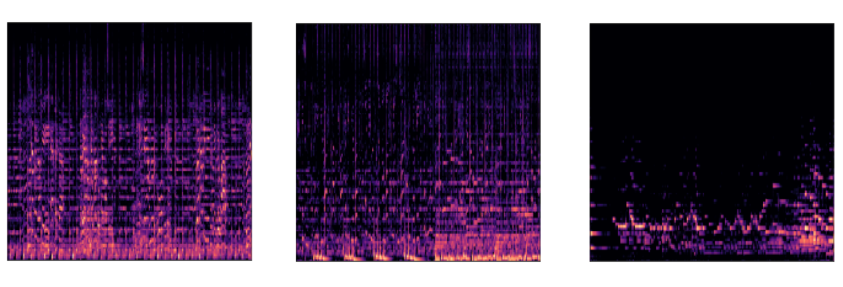
\includegraphics[scale=0.75]{spectrograms}
\caption{Primeri spektrograma}
\end{figure}

Skup podataka koji se koristi u ovom projektu već sadrzi odgovarajući spektrogram za svaku pesmu, potrebno je samo učitati podatke i izvršiti podelu na trening i test skup. Za test skup izdvojeno je 30\% podataka i to ravnomerno iz svake klase.

\subsubsection{Preprocesiranje .csv fajlova}

Fajlovi u formatu .csv sadrže razne odlike zvučnog signala u obliku tabele. Svakim redom u tabeli prikazane su odlike jedne pesme iz skupa. Atributi koji se mogu naći u njima su naziv i dužina pesme, ali i srednja vrednost i varijansa izračunate za različite podatke o zvuku poput frekvencije, harmonije, tempa i sl. Neophodno je ukloniti naziv pesme iz skupa atributa, s obzirom na to da je njegova vrednost jednistvena za svaku instancu.

Sve ostale vrednosti su neki realni brojevi, međutim nemaju iste raspodele. Kako ne želimo da dajemo nekim atributima veći značaj u odnosu na druge, potrebno je izvršiti standardizaciju podataka, tj. svođenje vrednosti svih atributa na standardnu normalnu raspodelu.

Standardizaciju je moguće izvršiti korišćenjem funkcije StandardScaler iz biblioteke sklearn. Pošto test podaci treba da budu nepoznati, kako bismo ispravno mogli da ocenimo kvalitet dobijenog modela, onda njihove vrednosti ne smeju uticati na matematičko očekivanje i standardnu devijaciju koji se koriste za skaliranje. Zbog toga je neophodno prvo izvršiti podelu na trening i test skup, a zatim StandardScaler prilagoditi samo trening podacima. Isti parametri se zatim koriste za transformaciju oba skupa.



\end{document}
